\subsection{DenseNet121 Model}
\label{subsec:densenet121}

DenseNet121 is a deep convolutional neural network architecture belonging to the family of Densely Connected Convolutional Networks (DenseNets), which were introduced by Huang \textit{et al.} in 2017 to address several limitations associated with traditional deep neural networks. DenseNet architectures were designed to improve feature propagation, encourage feature reuse, alleviate the vanishing gradient problem, and reduce the number of trainable parameters while maintaining high classification performance. Since its introduction, DenseNet121 has become one of the most widely adopted architectures in medical image analysis due to its ability to learn rich hierarchical representations from relatively limited datasets.

The fundamental idea behind DenseNet differs significantly from that of conventional convolutional neural networks. In traditional architectures, each layer receives information only from the immediately preceding layer and passes its output solely to the next layer. Although this sequential information flow is effective, it may lead to difficulties in gradient propagation as network depth increases. Furthermore, many learned feature maps become redundant because similar patterns are repeatedly relearned at different layers throughout the network.

To address these limitations, DenseNet introduces direct connections between layers. Instead of receiving input from only the previous layer, each layer receives the feature maps generated by all preceding layers within the same dense block. Consequently, information can flow directly from earlier layers to later layers without repeatedly passing through intermediate transformations. This dense connectivity pattern enables more efficient feature reuse and facilitates the training of very deep networks.

Figure~\ref{fig:densenet121_architecture} illustrates the overall architecture of DenseNet121.

\begin{figure}[H]
	\centering
	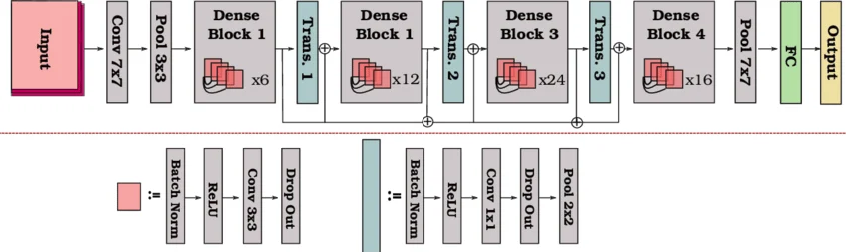
\includegraphics[width=\linewidth]{assets/DenseNet121.png}
	\caption{Overall architecture of DenseNet121 showing the arrangement of dense blocks, transition layers, and the final classification stage.}
	\label{fig:densenet121_architecture}
\end{figure}

\subsubsection{Motivation Behind Dense Connectivity}

As neural networks become deeper, the flow of information and gradients through the network becomes increasingly difficult. One of the most common challenges encountered in deep architectures is the vanishing gradient problem, where gradients become progressively smaller as they are propagated backward through many layers. When gradients become extremely small, early layers receive little useful learning signal, slowing convergence and potentially reducing overall performance.

Residual Networks (ResNets) partially addressed this issue through skip connections that allow gradients to bypass certain transformations. DenseNet extends this concept further by establishing direct connections between every pair of layers within a dense block. Instead of merely adding outputs from previous layers, DenseNet concatenates them. This strategy preserves information from all preceding layers and makes it directly accessible to subsequent layers.

The dense connectivity mechanism provides several important benefits. First, it improves gradient flow during training, allowing deeper networks to be optimized more effectively. Second, it encourages feature reuse, reducing redundancy among learned representations. Third, it improves parameter efficiency because layers can leverage previously learned features rather than learning entirely new representations from scratch.

\subsubsection{Dense Connectivity Mechanism}

The defining characteristic of DenseNet is the dense connection pattern between layers. Let $x_0$ represent the input to a dense block and let $x_l$ denote the output of the $l^{th}$ layer. Unlike traditional convolutional networks, where the output of layer $l$ depends only on the output of layer $l-1$, DenseNet computes each layer using the outputs of all preceding layers:

\begin{equation}
	x_l = H_l([x_0, x_1, x_2, ..., x_{l-1}])
\end{equation}

where:

\begin{itemize}
	\item $H_l(\cdot)$ denotes a composite transformation.
	\item $[\cdot]$ represents the concatenation operation.
	\item $x_0, x_1, ..., x_{l-1}$ are the feature maps generated by previous layers.
\end{itemize}

The concatenation operation differs fundamentally from the addition operation used in residual networks. Instead of merging features by summation, DenseNet preserves all previous feature maps and passes them directly to subsequent layers. As a result, each layer has access to both low-level and high-level information simultaneously.

This dense feature propagation mechanism allows later layers to exploit a richer collection of learned representations, improving feature diversity and reducing information loss.

\subsubsection{Dense Blocks}

The primary computational components of DenseNet121 are the dense blocks. A dense block consists of multiple densely connected layers arranged according to the connectivity pattern described previously.

Within each dense block, every layer receives as input the concatenated outputs of all preceding layers. Consequently, the number of feature maps grows progressively as additional layers are added. This growth is controlled through a parameter known as the \textit{growth rate}.

The growth rate, typically denoted by $k$, determines the number of new feature maps generated by each layer. If the input to a dense block contains $F_0$ feature maps and the block contains $L$ layers, the total number of feature maps at the end of the block can be expressed as:

\begin{equation}
	F = F_0 + kL
\end{equation}

where:

\begin{itemize}
	\item $F_0$ is the number of initial feature maps.
	\item $k$ is the growth rate.
	\item $L$ is the number of layers within the block.
\end{itemize}

For DenseNet121, the growth rate is typically set to 32. This means that each layer contributes 32 new feature maps while simultaneously utilizing all previously generated feature maps.

The use of a relatively small growth rate contributes to the parameter efficiency of DenseNet architectures, allowing them to achieve competitive performance with fewer parameters than many alternative architectures.

\subsubsection{Composite Function within Dense Layers}

Each layer within a dense block consists of a sequence of operations designed to transform incoming feature maps into more informative representations.

The composite transformation $H_l(\cdot)$ generally consists of:

\begin{enumerate}
	\item Batch Normalization (BN)
	\item Rectified Linear Unit (ReLU)
	\item Convolution
\end{enumerate}

This sequence is commonly referred to as the BN-ReLU-Conv pattern.

Batch normalization stabilizes the learning process by normalizing intermediate activations. This reduces internal covariate shift and allows higher learning rates to be used during training.

The ReLU activation function introduces non-linearity into the network and is defined as:

\begin{equation}
	f(x) = \max(0,x)
\end{equation}

Following activation, convolutional filters extract spatial patterns from the input feature maps. Through repeated application of these operations, the network gradually learns increasingly abstract representations of the input image.

\subsubsection{Bottleneck Layers}

As the number of feature maps grows within dense blocks, computational complexity can increase significantly. To reduce this cost, DenseNet121 employs bottleneck layers.

A bottleneck layer consists of a $1 \times 1$ convolution applied before the standard $3 \times 3$ convolution. The purpose of this operation is to reduce the number of feature channels while preserving important information.

The bottleneck structure can be summarized as:

\begin{equation}
	BN \rightarrow ReLU \rightarrow Conv(1\times1)
	\rightarrow BN \rightarrow ReLU \rightarrow Conv(3\times3)
\end{equation}

The use of bottleneck layers substantially reduces computational requirements while maintaining representational capacity.

\subsubsection{Transition Layers}

Because feature map dimensions increase continuously within dense blocks, DenseNet introduces transition layers between consecutive blocks to control network complexity.

A transition layer performs two primary functions. First, it reduces the number of feature maps through a $1 \times 1$ convolution. Second, it decreases spatial resolution using average pooling.

The transition layer architecture typically follows:

\begin{equation}
	BN \rightarrow ReLU \rightarrow Conv(1\times1)
	\rightarrow AvgPool(2\times2)
\end{equation}

These operations prevent excessive growth in memory consumption while preserving the most informative features.

Transition layers also contribute to hierarchical feature extraction by gradually reducing spatial dimensions as network depth increases.

\subsubsection{Architecture of DenseNet121}

DenseNet121 consists of four dense blocks separated by three transition layers. The architecture begins with an initial convolution layer and concludes with global average pooling followed by a fully connected classification layer.

The distribution of layers across dense blocks is as follows:

\begin{table}[H]
	\centering
	\caption{Layer distribution within DenseNet121.}
	\begin{tabular}{|c|c|}
		\hline
		Component & Number of Layers \\
		\hline
		Dense Block 1 & 6 \\
		Dense Block 2 & 12 \\
		Dense Block 3 & 24 \\
		Dense Block 4 & 16 \\
		\hline
		Total Dense Layers & 58 \\
		\hline
	\end{tabular}
	\label{tab:densenet121_blocks}
\end{table}

When all convolutional, pooling, and classification layers are included, the network contains 121 trainable layers, which gives the architecture its name.

The input image first passes through an initial $7\times7$ convolution layer followed by max pooling. Feature extraction then proceeds through the sequence of dense blocks and transition layers. Finally, global average pooling aggregates spatial information into a compact feature vector, which is passed to the final classification layer.

\subsubsection{Advantages of DenseNet121 for Medical Image Analysis}

DenseNet121 possesses several characteristics that make it particularly suitable for medical image classification tasks.

The dense connectivity pattern encourages extensive feature reuse, allowing the network to learn robust representations even when training datasets are relatively small. This characteristic is especially important in medical imaging, where acquiring large annotated datasets is often challenging.

The improved gradient flow resulting from dense connections facilitates stable optimization and reduces the risk of vanishing gradients. Consequently, deeper representations can be learned without the training difficulties commonly associated with very deep neural networks.

DenseNet121 is also highly parameter-efficient compared to many competing architectures. Despite its depth, the network requires fewer trainable parameters than several traditional convolutional architectures because previously learned features are reused rather than repeatedly regenerated.

Furthermore, the architecture has demonstrated strong performance across a wide range of medical imaging applications, including chest disease classification, pneumonia detection, COVID-19 diagnosis, tuberculosis screening, diabetic retinopathy analysis, and cancer detection. Its proven effectiveness in healthcare applications has made DenseNet121 a popular backbone network for medical image analysis research.

\subsubsection{DenseNet121 in the Proposed Framework}

In the context of this work, DenseNet121 was selected as the backbone architecture for the first-level routing model due to its strong balance between classification performance, computational efficiency, and feature extraction capability. The dense connectivity structure enables the model to capture both low-level radiological patterns and high-level pathological characteristics that are essential for accurate disease recognition.

Additionally, the feature reuse mechanism of DenseNet121 is particularly advantageous for medical datasets, where image variability can be substantial and labeled samples may be limited. By leveraging information from all preceding layers, the network can construct rich hierarchical representations that support robust classification performance.

Overall, DenseNet121 provides a powerful and efficient deep learning architecture that aligns well with the requirements of medical image analysis systems. Its dense connectivity, parameter efficiency, strong gradient propagation, and proven effectiveness in healthcare applications make it an appropriate choice for the disease classification tasks addressed in this project.